\chapter{Dataset Construction}
\label{chap:dataset-construction}


% -------------------------------------------------------------------
% Data Collection
% -------------------------------------------------------------------
\section{Data Collection}
\label{sec:data-collection}

To serve our dedicated approach, we have to handle textual data that are reviews on E-commerce platforms. We choose Scrapy\footnote{\url{https://scrapy.org/}} to crawl the data from online shopping websites including \url{http://www.tiki.vn} and \url{http://www.shopee.vn}. They are two of Vietnam's most common and trusted e-commerce platforms.
We focus on technology and mother \& baby domains since they are the most interested domain in Vietnamese e-commerce.
These raw data are then used as input for Data Annotation step that we will describe in Section~\ref{sec:data-annotation}.

% -------------------------------------------------------------------
% Data Annotation
% -------------------------------------------------------------------
\section{Data Annotation}
\label{sec:data-annotation}
\begin{table}[]
\centering
\resizebox{\linewidth}{!}{
\begin{tabular}{|c|c|>{\raggedright\arraybackslash}m{11 cm}|}
\hline
\textit{\textbf{Domain}}                         & \textit{\textbf{Aspect}} & \multicolumn{1}{c|}{\textit{\textbf{Description}}}                                                                                                                                                                \\ \hline
\multirow{8}{*}{\textbf{Technology}} & Price                    & Cut/ reduce/ slash/ low price considered positive while increase/ put up/ raise/ high price is considered negative.                                            \\ \cline{2-3} 
                               & Service                  & Nice, fast, efficient, enthusiastic support is considered positive while no reply, irresponsibility or carelessly packing is considered negative.                                                                 \\ \cline{2-3} 
                               & Delivery                & The quality, speed and cost of shipping process. If it is fast, carefully shipped and the cost is low, it is considered positive, otherwise is negative.                                                          \\ \cline{2-3} 
                               & Performance              & Fast processing speed is considered positive while lag or latency in the middle of an app or apps shut down unexpectedly is considered negative.                      \\ \cline{2-3} 
                               & Hardware                 & The quality of the hardware of the device including display, chip, battery, cameras, storage, RAM, etc.                                                                                                           \\ \cline{2-3} 
                               & Authenticity             & Genuinely produced product is considered positive while fake, imitation is consider negative.                                                                                                                      \\ \cline{2-3} 
                               & Accessories              & Fully provided, good quality accessories are considered positive; low quality or missed are considered negative.                                                            \\ \cline{2-3} 
                               & Appearance               & Product with nice design, nice color, luxury, etc. are considered positive, product with scratches, awful design is consider negative.                                                                             \\ \hline
\multirow{6}{*}{\textbf{Mother \& Baby}}     & Price                    & Cut/ reduce/ slash/ low price considered positive while increase/ put up/ raise/ high price is considered negative.                                            \\ \cline{2-3} 
                               & Service                  & Nice, fast, efficient, enthusiastic support  is considered positive while no reply, irresponsibility or carelessly packing is considered negative.                                                                 \\ \cline{2-3} 
                               & Delivery               & The quality, speed and cost of shipping process. If it is fast, carefully shipped and the cost is low, it is considered positive, otherwise negative.                                                             \\ \cline{2-3} 
                               & Safety                   & Product having obvious expiration date and has not expired, safe to use is considered positive, while product that is expired or causes allergy, rashes is considered negative. \\ \cline{2-3} 
                               & Quality                  & Customer experience on the product: the softness, absorbency of diapers, the taste and smell of milk, etc.                                                                                                        \\ \cline{2-3} 
                               & Authenticity             & Genuinely produced product is considered positive while fake, imitation is consider negative.                                                                                                                      \\ \hline
\end{tabular}
}
\caption{Aspect description}
\end{table}

We used Docanno as a tool for data annotation. First of all, we overview the data set collected from crawling process to figure out aspects that were frequently mentioned on users’ reviews. 

After discussion, we extracted aspect terms in the sentences and labeled the sentiment polarities with respect to the aspect terms using Docanno. Table 1 illustrates how we handle each aspect. For Technology domain, we predefined eight coarse aspect categories: price, service, delivery, performance, hardware, authenticity, accessories, design. For Mother \& Baby, these are: price, service, delivery, safety, quality and authenticity. In each aspect, it is considered negative when there is at least a complaint regarding that aspect, otherwise it is considered negative.

\begin{figure}[h]
	\centering
	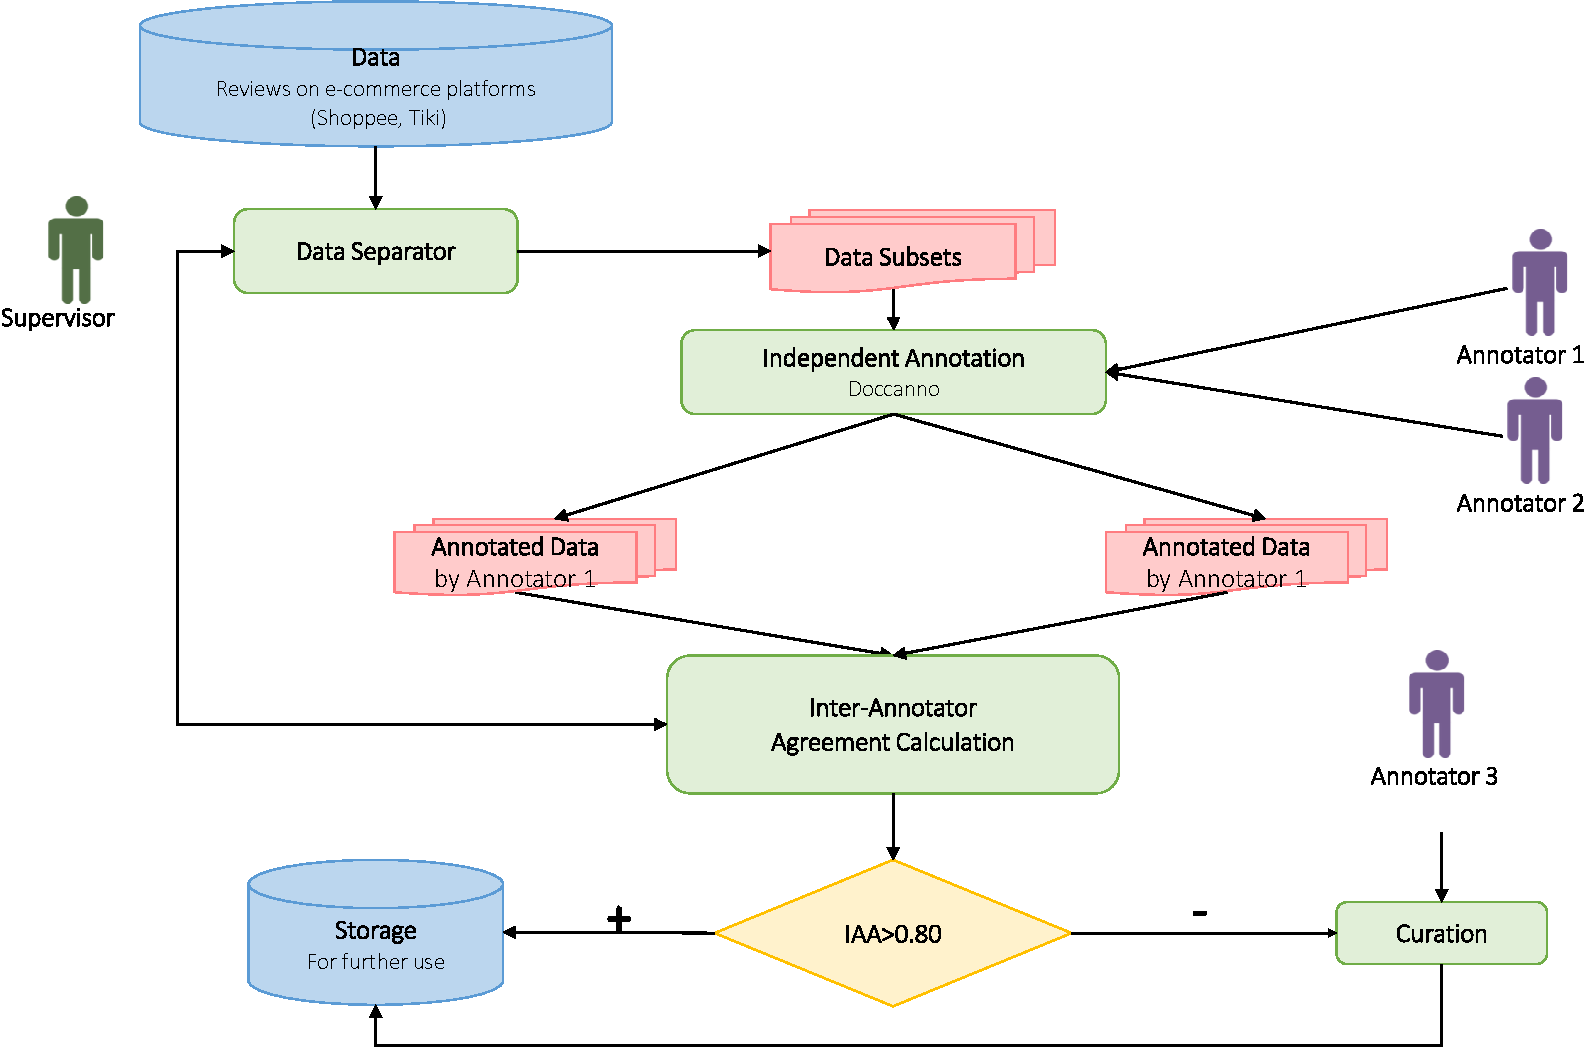
\includegraphics[width=\linewidth]{Chapter2/Figs/annotation.pdf}
	\caption{Data Annotation process}
	\label{fig:annotation}
\end{figure}

Data then separated in subsets, each of them was then evaluated and labeled by 2 annotators independently. Next, we measured the agreement between two annotators, if the result is too low (Inter-Annotator Agreement or IAA \(<\) 0.8), manually reviewing – process will be applied. The labeled data then stored as input for Pre-processing step. 

% -------------------------------------------------------------------
% Dataset Analysis
% -------------------------------------------------------------------
\section{Dataset Analysis}
\label{sec:data-analysis}
\paragraph{}
The statistics of Vietnamese E-commerce dataset (VECD) including Shopee and Tiki in two different domains:  Technology and Mother \& Baby are reported in figure 1 to 4. VECD consists of 3016 instances of Shopee Mother \& Baby, 2986 instances of Tiki , 3002 instances of Shopee Technology and 3236 instances of Tiki Technology, making up 12240 instances in total.

\begin{table}[h]
\centering
\begin{tabular}{|l|c|c|c|c|}
\hline
\multirow{2}{*}{}                                        & \multicolumn{2}{c|}{\textbf{Mother \& Baby}}           & \multicolumn{2}{c|}{\textbf{Technology}}                \\ \cline{2-5} 
                                                         & \textit{\textbf{Shopee}} & \textit{\textbf{Tiki}} & \textit{\textbf{Shopee}} & \textit{\textbf{Tiki}} \\ \hline
\multicolumn{1}{|c|}{\textbf{Total aspect}}              & 6                        & 6                      & 8                        & 8                      \\ \hline
\multicolumn{1}{|c|}{\textbf{Aspect count per sentence}} & 1.753234                 & 1.497347               & 2.087627                 & 1.746551               \\ \hline
\end{tabular}
\caption{The average number of aspects mentioned}
\end{table}

\begin{figure}[h]
	\centering
	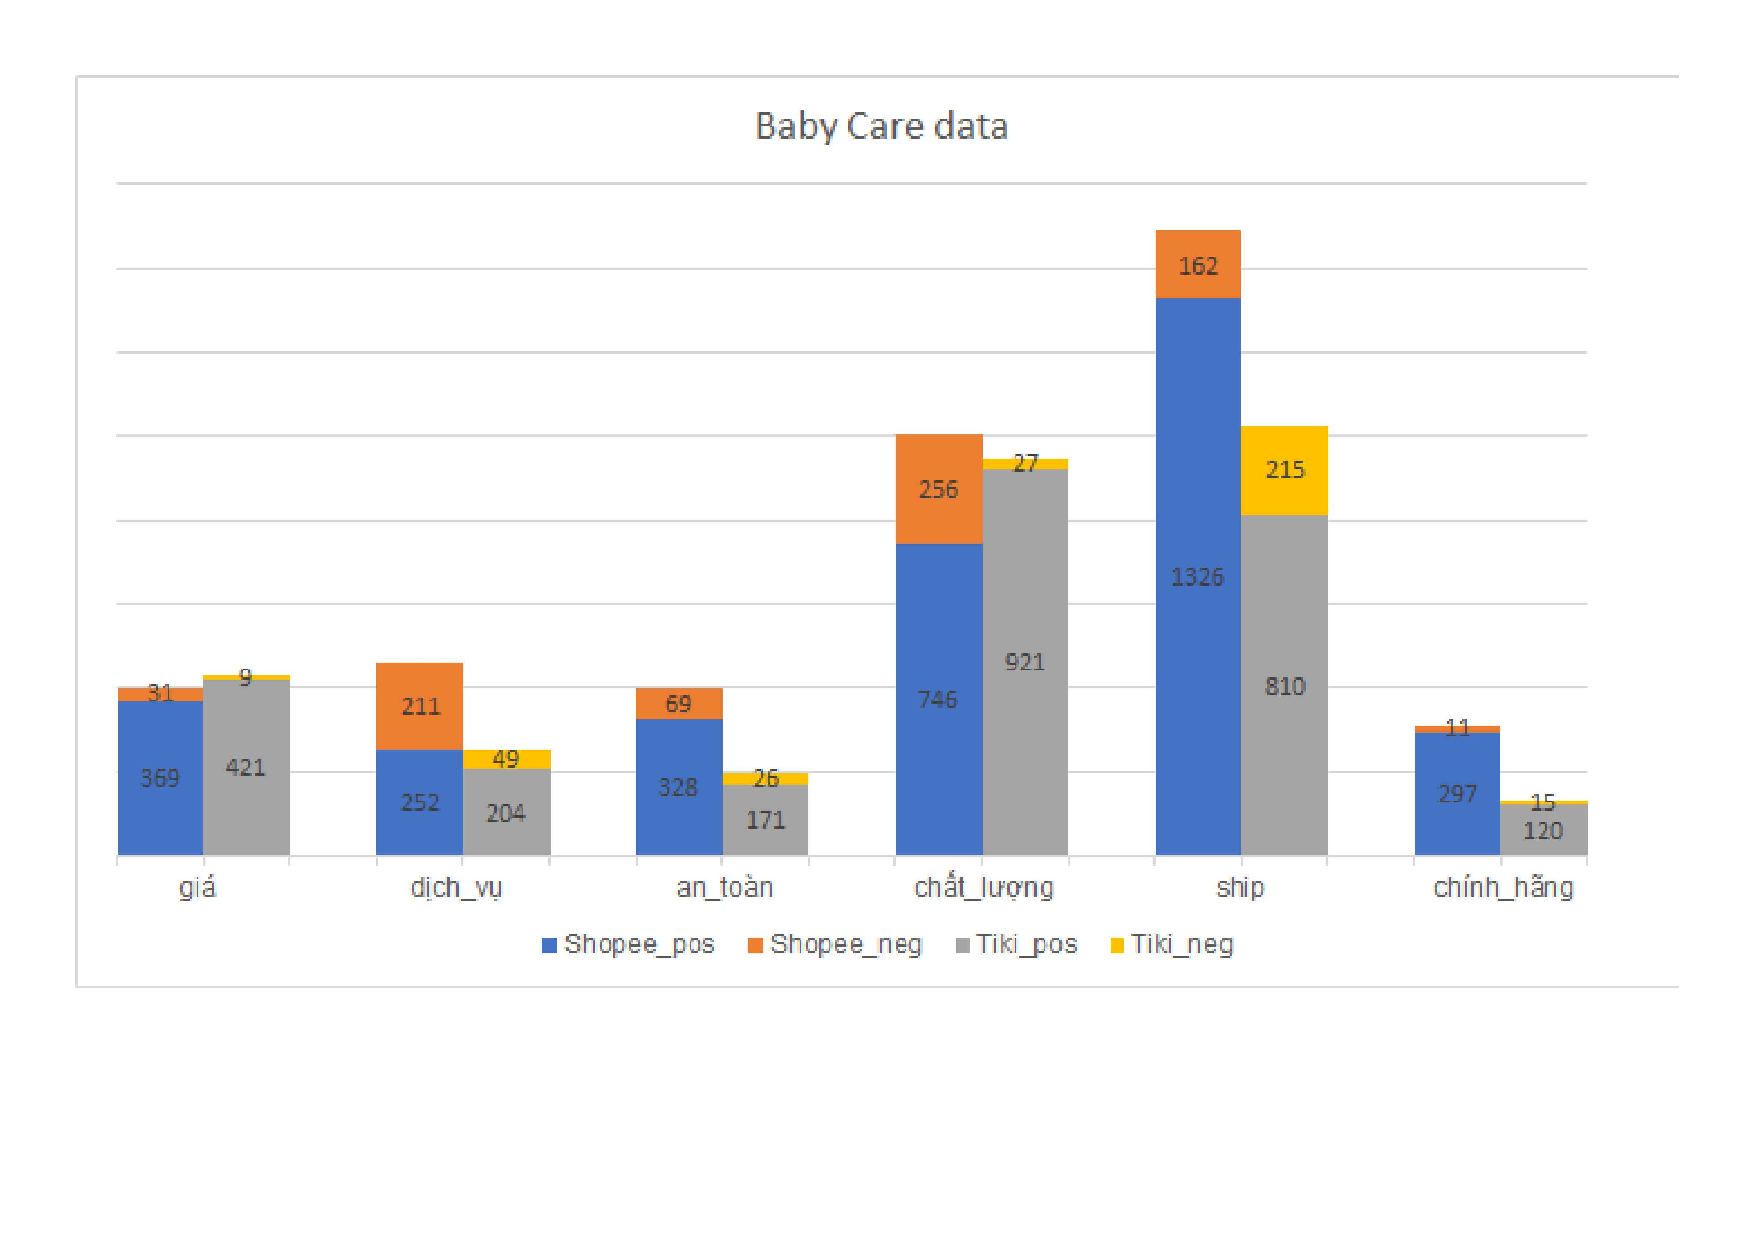
\includegraphics[width=\linewidth]{Chapter2/Figs/baby care.pdf}
	\caption{Mother \& Baby data statistics}
	\label{fig:baby}
\end{figure}

In Mother \& Baby domain, Shipping and Quality appear to be the most concerned aspects. Shopee has $1541$/$3216$ comments on Shipping and $773$/$3216$ comments on Quality, while in Tiki they are $972$/$2986$ and $1177$/$2986$ respectively. Authenticity only occasionally mentioned in Tiki's comments, just in $131$ cases while the others are mentioned in over $200$ comments, in both platforms, including Authenticity mentioned in Shopee.

Similarly, in Technology domain, Appearance is frequently mentioned in Shopee while it is Shipping in Tiki. More specifically $1064$ out of $3002$ comments on Shopee have information relating to products’ appearance, compared to $1021$ out of $3236$ comments on Tiki having information about Shipping. Price and Authenticity are the most imbalanced aspects, with only $4$ negative comments on Price and $12$ negative comments on Authenticity in Shopee while in Tiki the figures are $31$ and $24$, respectively. In Tiki, although the number of comments on Service, Hardware, Performance and Accessories is comparatively low, the data on these aspects are relatively balanced, with the difference below $16\%$.

\begin{figure}[]
	\centering
	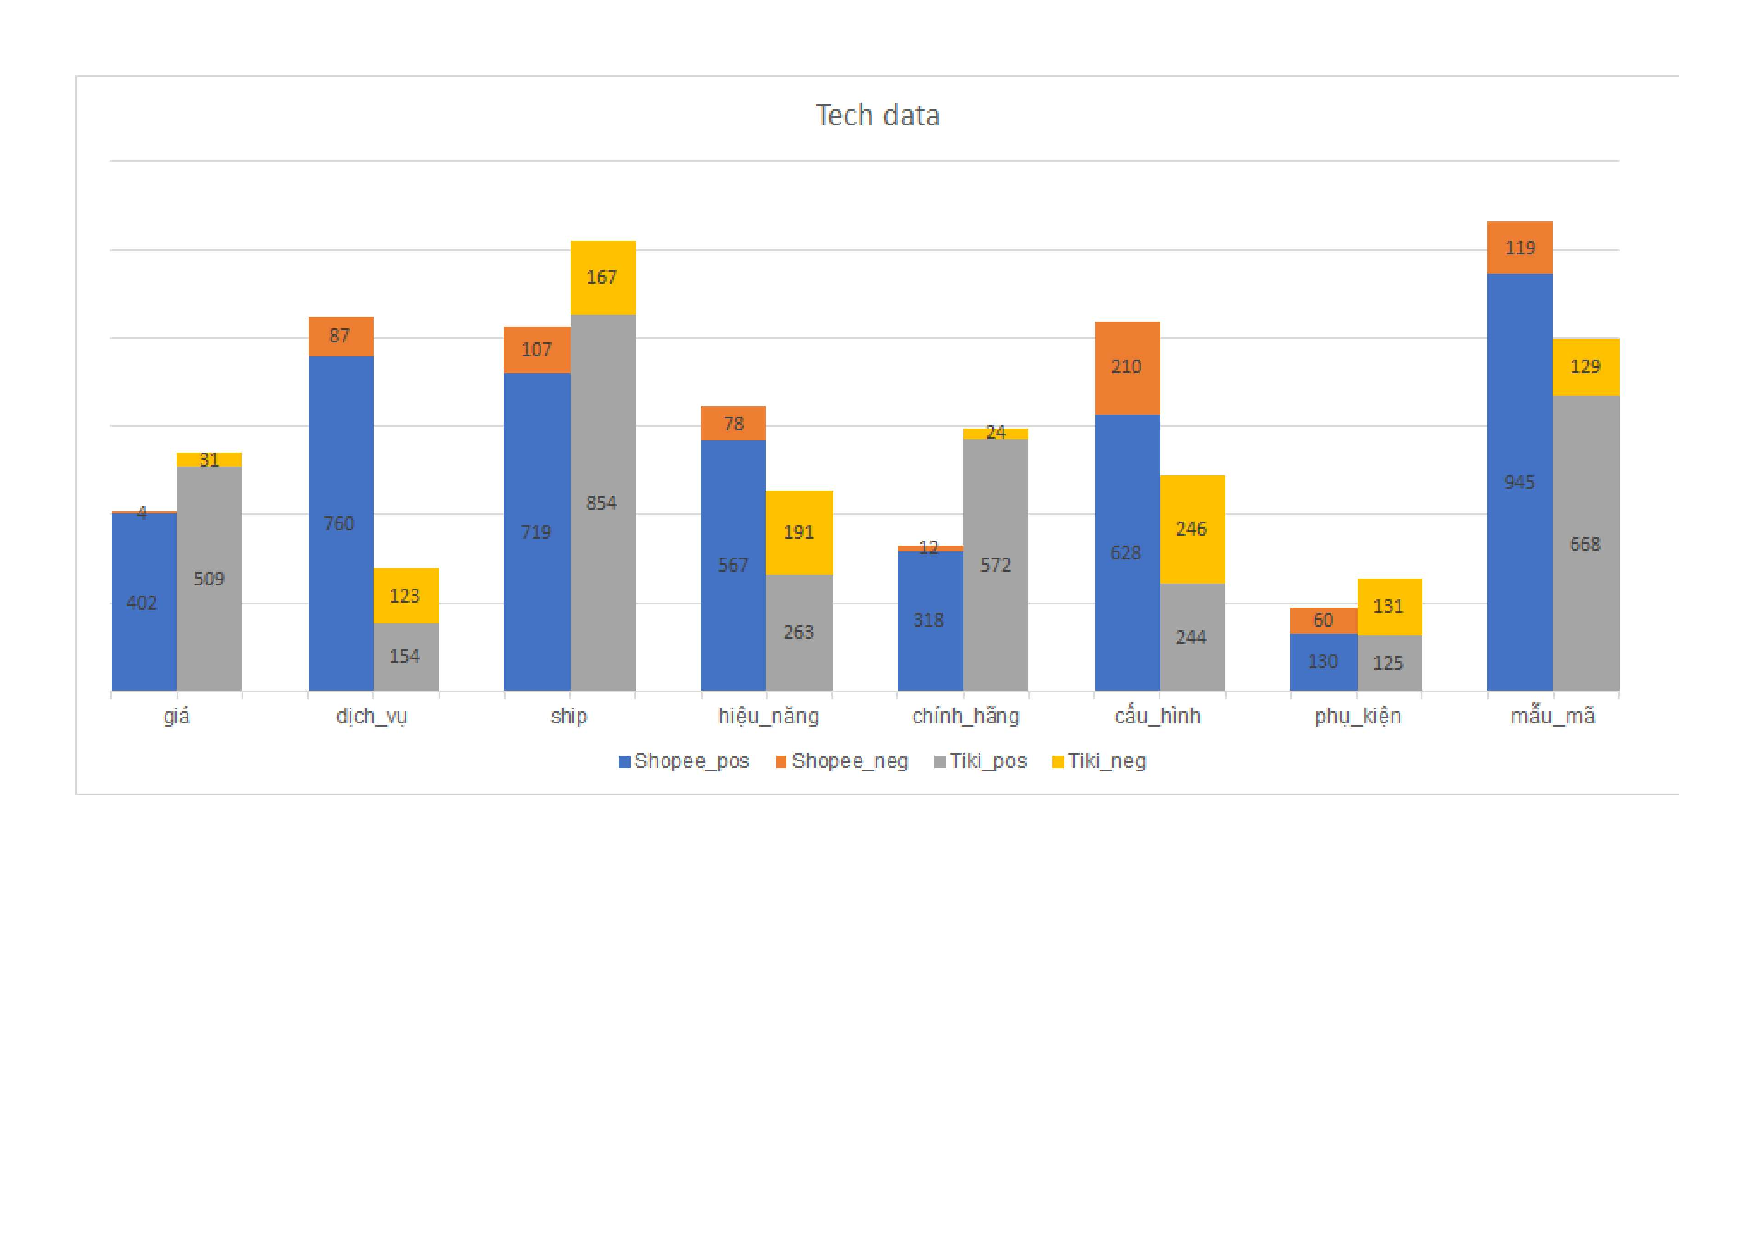
\includegraphics[width=\linewidth]{Chapter2/Figs/tech data.pdf}
	\caption{Technology data statistics}
	\label{fig:tech}
\end{figure}












